\section{Components}
\label{sec:components}
Just like in Unity, the components are the building blocks of the game objects.
They are the individual features that can be added to a game object to give it functionality.

\subsection{class diagram}
\begin{figure}[H]
    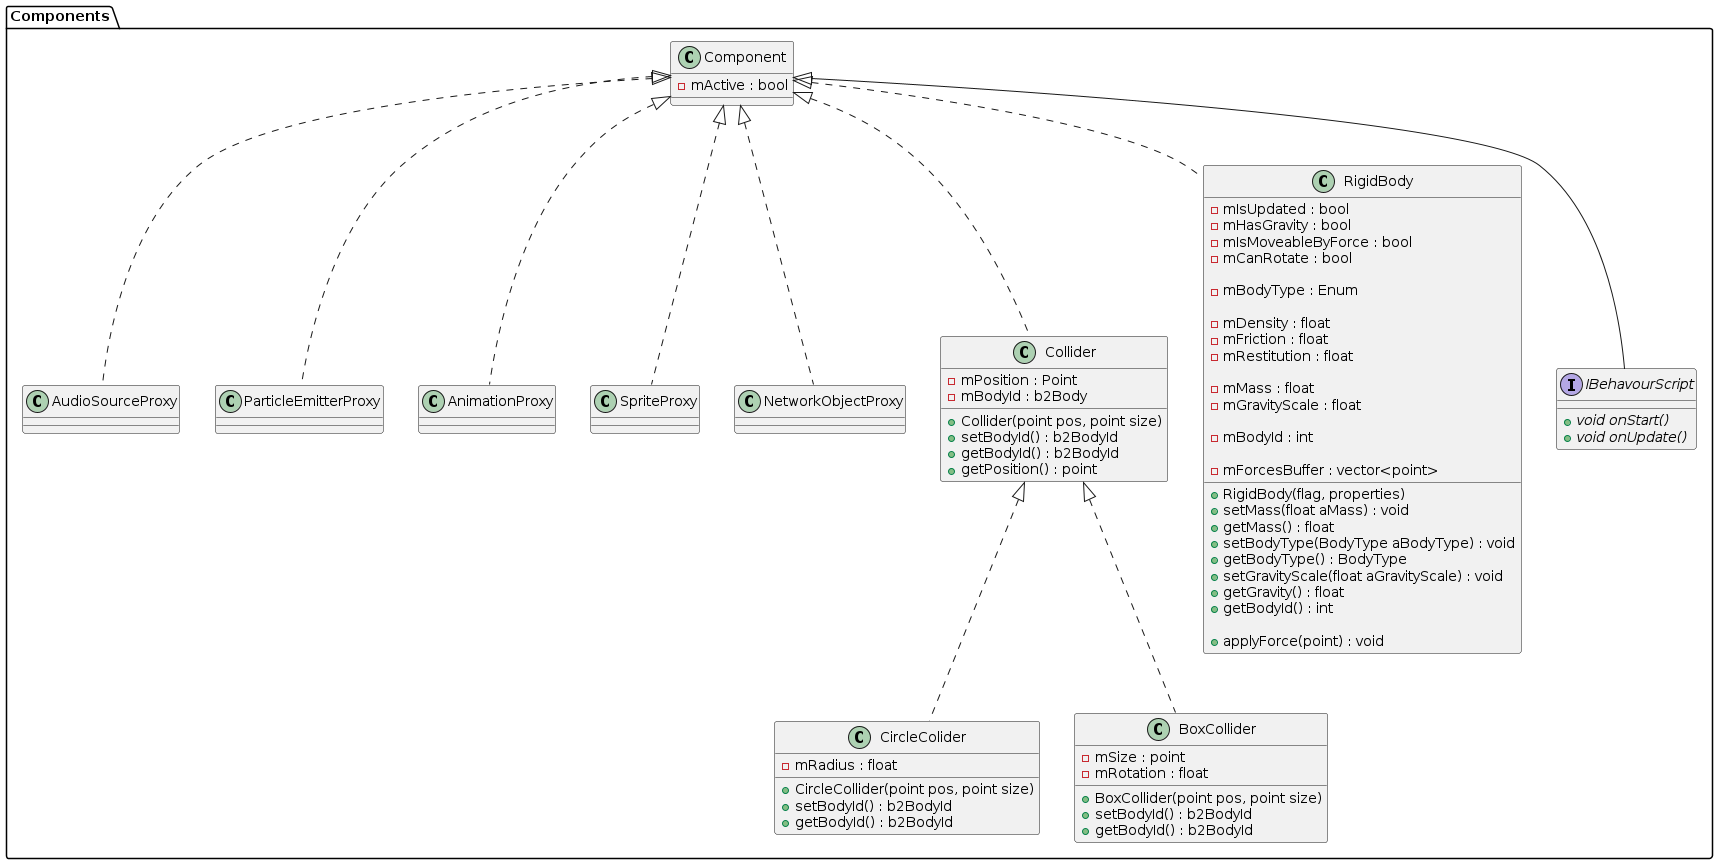
\includegraphics[width=1.2\textwidth]{componentsPackageClassDiagram.png}
    \caption{Class diagram of the components}
    \label{fig:components}
\end{figure}

\subsection{AudioSourceProxy}
See \autoref{sec:audio} for more information.
Used to add audio to a GameObject.

\subsection{ParticleEmitterProxy}
See \textbf{TODO: add reference to particle emitter}
Used to create particle effects.

\subsection{AnimationProxy}
See \textbf{TODO: add reference to Animation emitter}

\subsection{SpriteProxy}
See \textbf{TODO: add reference to Sprite emitter}

\subsection{Collider}
Has \texttt{bodyID}, which is needed for the physics.

\subsection{NetworkObjectProxy}
see \autoref{sec:networking} for more information.

\subsection{Sprite}
Used to add a still image to a GameObject.
The Sprite Component has the following properties:
\begin{itemize}
    \item \texttt{texture} - The texture of the sprite.
    \item \texttt{width} - The width of the sprite.
    \item \texttt{height} - The height of the sprite.
    \item \texttt{flipx} - Whether the sprite is flipped horizontally.
    \item \texttt{flipy} - Whether the sprite is flipped vertically.
    \item \texttt{sprite source} - The source rectangle that defines which part of the texture is rendered(can be set to 0 to render all).
    \item \texttt{transform.x} - The x position of the texture relative to the GameObject it is attached to.
    \item \texttt{transform.y} - The y position of the texture relative to the GameObject it is attached to.
    \item \texttt{transform.rotation} - The rotation of the texture relative to the GameObject it is attached to.
\end{itemize}

\subsection{Animation}
Used to add an animated image to a GameObject.
The Animation Component has the following properties:
\begin{itemize}
    \item \texttt{sprites} - The sprites that make up the animation.
    \item \texttt{transform.x} - The x position of the animation relative to the GameObject it is attached to.
    \item \texttt{transform.y} - The y position of the animation relative to the GameObject it is attached to.
    \item \texttt{transform.rotation} - The rotation of the animtion relative to the GameObject it is attached to.
    \item \texttt{flipX} - Whether the animation is flipped horizontally.
    \item \texttt{flipY} - Whether the animation is flipped vertically.
    \item \texttt{frameCount} - The amount of frames in the animation.
    \item \texttt{frameTime} - The time between each frame.
    \item \texttt{currentFrame} - The current frame of the animation.
    \item \texttt{loop} - Whether the animation should loop.
\end{itemize}
\subsection{Collider}

\subsection{CircleCollider}

\subsection{BoxCollider}

\subsection{RigidBody}
Has \texttt{bodyID}, which is needed for the physics.

\subsection{IBehaviourScript}
IBehaviour script is an interface that can be used to create behaviour scripts for GameObjects.

\subsection{ParticleEmitter}
Particle emitter is a component that can be used to create particle effects.
The particle emitter has the following properties:
\begin{itemize}
    \item \texttt{particles} - The particles that make up the particle effect.
    \item \texttt{transform.x} - The x position of the particle effect relative to the GameObject it is attached to.
    \item \texttt{transform.y} - The y position of the particle effect relative to the GameObject it is attached to.
    \item \texttt{transform.rotation} - The rotation of the particle effect relative to the GameObject it is attached to.
    \item \texttt{angle} - in which direction the particles are emitted.
    \item \texttt{emissionRate} - The amount of particles emitted per second.
    \item \texttt{particleLifetime} - The lifetime of the particles.
    \item \texttt{particleSpeed} - The speed of the particles.
    \item \texttt{particleSize} - The size of the particles.
    \item \texttt{particleSizeShift} - The shift in size of the particles.
    \item \texttt{particleColor} - The color of the particles.
    \item \texttt{rotationSpeed} - The speed at which the particles rotate.
    \item \texttt{acceleration} - The acceleration of the particles.
    \item \texttt{angularAcceleration} - The angular acceleration of the particles.
\end{itemize}

\subsection{AudioSource}
Used to add audio to a GameObject. See chapter \autoref{sec:audio} for details

\subsection{Transform}
The Transfrom is not a class but a struct. It represents the position, rotation and scale of a GameObject.
Does not need an update flag when the position is changed, as a movable object is usually moving.


